\documentclass{sig-alternate}
\usepackage{graphicx,url,amsmath,amsfonts,amssymb,color,multirow}

\pagestyle{empty}

\def\sharedaffiliation{
\end{tabular}
\begin{tabular}{c}}

\tolerance 400
\setlength{\emergencystretch}{3em}

\begin{document}

\conferenceinfo{MobiSys'10,} {June 15--18, 2010, San Francisco, California, USA.} 
\CopyrightYear{2010}
\crdata{978-1-60558-985-5/10/06}

\title{IDEA: Integrated Distributed Energy Awareness\\for Wireless Sensor Networks}
\numberofauthors{3}

\author{
\alignauthor Geoffrey Werner Challen\\
\email{challen@eecs.harvard.edu}
\alignauthor Jason Waterman\\
\email{waterman@eecs.harvard.edu}
\alignauthor Matt Welsh\\
\email{mdw@eecs.harvard.edu}
\sharedaffiliation
\affaddr{School of Engineering and Applied Sciences}\\
\affaddr{Harvard University}\\
\affaddr{Cambridge, MA}
}

\maketitle

\begin{abstract}

Energy in sensor networks is a distributed, non-transferable resource. Over
time, differences in energy availability are likely to arise. Protocols like
routing trees may concentrate energy usage at certain nodes. Differences in
energy harvesting arising from environmental variations, such as if one node
is in the sun and another is in the shade, can produce variations in charging
rates and battery levels. Because many sensor network applications require
nodes to collaborate --- to ensure complete sensor coverage or route data to
the network's edge --- a small set of nodes whose continued operation is
threatened by low batteries can have a disproportionate impact on the
fidelity provided by the network as a whole. In the most extreme case, the
loss of a single sink node may render the remainder of the network
unreachable.

While previous research has addressed reducing the energy usage of individual
nodes, the challenge of collaborative energy management has been largely
ignored. We present Integrated Distributed Energy Awareness (IDEA), a sensor
network service enabling effective network-wide energy decision making. IDEA
\textit{integrates} into the sensor network application by providing an API
allowing components to evaluate their impact on other nodes. IDEA
\textit{distributes} information about each node's load rate, charging rate,
and battery level to other nodes whose decisions affect it. Finally, IDEA
enables \textit{awareness} of the connection between the behavior of each
node and the application's energy goals, guiding the network toward states
that improve performance.

This paper describes the IDEA architecture and demonstrates its use through
three case studies. Using both simulation and testbed experiments, we
evaluate each IDEA application by comparing it to simpler approaches that do
not integrate distributed energy awareness. We show that using IDEA can
significantly improve performance compared with solutions operating with
purely local information.

\end{abstract}

\vfill\eject

\category{C.2.4}{Computer-Communication Networks}{Distributed Systems}
\category{C.3}{Special-Purpose and Application-Based Systems}{Real-time and
Embedded Systems}
\terms{Design}
\keywords{Wireless Sensor Networks, Resource Management, Resource
Distribution, Optimization}

\section{Introduction}
\label{sec-introduction}

Energy-harvesting sensor networks experience variations in load and charging
rates that threaten high-fidelity operation. Changing application demands
produce variations in load rates, while energy-harvesting properties
produce variations in charging rates. Energy mismanagement can lead to
reduced fidelity, when nodes' batteries empty, or wasted energy, when nodes
harvest energy they cannot store.

Energy harvesting capabilities --- such as solar charging --- further
complicate the distributed energy management task. The energy collected at
each node may vary significantly based on node placement, and the energy
collected daily may vary significantly based on weather patterns.  Preparing
the network for overnight operation requires capturing as much energy as
possible during the day and minimizing energy wasted charging full batteries,
while overnight operation requires adjusting the network's load profile to
match the distribution of energy stored during daytime.

Fortunately, dense networks provide redundancy that can be used to control
the distribution of energy usage. Multiple possible routing paths may connect
a node to the sink. Tuning MAC parameters allows nodes to shift communication
load to their neighbors. Sensor inputs from multiple nodes may be redundant,
allowing some to be disabled or operated at reduced fidelity.  The existence
of these choices implies that it is possible to tune the energy load of the
network to better match energy availability. Effective load tuning can
increase the fidelity provided to the application at a fixed battery size, or
allow battery sizes to be reduced while maintaining the required fidelity
level.
\vfill\eject

Existing sensor network platforms provide little support for collaborative
energy management. Approaches such TinyOS~\cite{tinyos-asplos00},
Pixie~\cite{pixie-sensys08}, Eon~\cite{eon-sensys07}, and
Levels~\cite{levels-sensys07} facilitate local control only, failing when
greedy node energy minimization fails to produce the best outcome.
Network-wide solutions such as Lance~\cite{lance-sensys08},
Mercury~\cite{parkinsons-embs07}, and EnviroMic~\cite{enviromic} either
require centralized control or are tailored to the needs of a specific
application domain. In sensor networks the majority of energy consumption is
consumed by multi-node collaboration. We argue that due to the distributed
nature of energy consumption and availability, improving performance requires
consideration of both \textit{where} energy is and \textit{how much} is being
used.

Matching load to availability across the network requires
\textit{integrating} with application components producing energy load,
\textit{distributing} load and availability information to facilitate node
decision making, and \textit{awareness} of the connection between load,
availability, and application-level fidelity. In this paper, we propose
\textit{Integrated Distributed Energy Awareness (IDEA)}, a sensor network
service addressing these goals. IDEA monitors and models the load and charge
rates on each node. To allow nodes to reason about their impact on others,
each node distributes its model parameters, updating them as necessary to
ensure continued accuracy. IDEA clients are responsible for estimating their
own distributed energy impact. When changing state, IDEA helps them evaluate
each proposed option using an energy objective function tailored to meet
specific application goals. By tracking availability and informing the energy
decision-making process, IDEA simplifies the construction of energy-aware
components.

Our paper makes the following contributions. First, we describe IDEA, a new
service uniting energy monitoring, load modeling, and distributed data
sharing into a single service facilitating distributed decision making.
Second, we present three case studies illustrating how to use IDEA, including
a component that tunes MAC parameters, an existing routing protocol modified
to choose energy-aware routes, and an application using IDEA to determine how
to localize acoustic events. Third, using simulation and testbed results we
compare the performance of IDEA with approaches that do not consider energy
distribution, showing that IDEA enables improvements in lifetime of up to
35\%.

The rest of this paper is organized as follows. Section~\ref{sec-motivation}
motivates the need for IDEA using a simple example. In
Section~\ref{sec-architecture} we present the IDEA architecture in detail and
describe our current implementation. We describe our three case studies in
detail in Section~\ref{sec-casestudies}. Section~\ref{sec-evaluation}
presents simulation and testbed results. We review related work in
Section~\ref{sec-related}, and Section~\ref{sec-futurework} outlines future
work and concludes.

\section{Motivation}
\label{sec-motivation}

IDEA's architecture is motivated by two observations. First, many sensor
network applications require a large portion of the network to meet their
fidelity requirements. As a result, failures of sensor nodes can deeply
impact delivered data quality. Indeed, the most heavily-loaded nodes are
often those that are most critical to the application. Consider a node near
the root of a spanning tree, which is responsible for forwarding traffic for
a substantial portion of the network. Loss of this single node can have a
disproportionate effect on the whole network's operation.
\vfill\eject

Second, in most applications, some portion of the load at each node is due to
interaction with other nodes and cannot be reduced unilaterally. In the case
of routing, nodes spend their own energy to listen to and forward packets for
other nodes. In such cases, load mitigation must be negotiated with the peer
nodes producing the load. For example, a node with a valuable sensor input
might do everything possible to reduce its own power consumption, but unless
it can move itself off of a high-traffic routing path, it will be unable to
reduce energy expenditure beyond a certain point.

Existing approaches to sensor network energy management suffer from several
weaknesses. Greedy approaches to local energy minimization assume that each
node minimizing its own power consumption is best for the network as a whole.
However, this is not always the case. Such approaches also cannot address the
external load problem described above. Some sensor network protocols embed
forms of distributed energy management into their operation, but by doing so
they encode policies unsuitable for certain applications. IDEA addresses
these deficiencies by providing a distributed service allowing any component
controlling distributed load to perform collaborative energy management.

\subsection{Example: Energy-Aware Routing}

\begin{figure}[t]
\begin{center}
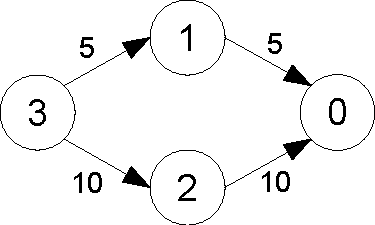
\includegraphics[width=0.9\hsize]{./figs/MotivationExample.pdf}
\end{center}

\caption{\textit{Example routing problem.} The edges are the energy in
mJ to send a packet.}

\label{fig-motivationexample}
\end{figure}

As a simple example demonstrating the need for IDEA, consider a four-node
routing problem. Figure~\ref{fig-motivationexample} shows the network
topology, with the energy required to reliably transfer a packet over each
link shown. (To simplify the example we ignore receive costs, assume all
nodes have the same data rate of one packet per second, and assume a powered
sink.) The application attempts to localize events by collecting data from
the network, and must use all four nodes, meaning that the loss of a single
node will render the network useless.

Node~3 has two routes to the sink Node 0: $3,1,0$ and $3,2,0$. If Node~3
conserves power by making a local greedy decision, it will route through
Node~1, since sending a packet to Node~1 consumes $0.5$~mJ of energy as
opposed to $1.0$~mJ for sending to Node~2. Even assuming Node~3 knows the
power consumption of the links $1,0$ and $2,0$, with no other information it
still chooses the route though Node~1, which consumes less total energy per
packet than the route through Node~2, 1.0~mJ per packet versus 2.0~mJ.

\vfill\eject

The question we ask is, under what conditions will using route $3,1,0$ ---
which consumes the least energy locally and globally --- actually
\textit{harm} application performance?  We identify four situations where
using the alternative route $3,2,0$ is the correct choice, each described
below. To facilitate our discussion we define $B_n$, $C_n$ and $L_n$ as the
battery in joules, charging rate in mJ per second, and non-routing load
in mJ per second at Node $n$ respectively. The choice we are considering
is between two possible load distributions, $R \in \mathcal{R}$, where
$R^{3,1,0} = (0.0, 1.0, 1.0, 0.5)$ and $R^{3,2,0} = (0.0, 0.5, 2.0, 1.0)$.
$R^{Route}_n$ represents the cost to Node $n$ assuming Node 3 uses the route
indicated. (Node~1 and Node~2 route directly to the sink.)  For example,
$R^{3,2,0}_2$ is 2.0 mJ because the cost to send a packet from Node~2 to
Node~0 is 1.0 mJ and Node~2 must send two packets, one from Node~3 as well as
a packet from the data generated locally at Node~2.

\vspace{0.1in}

\begin{itemize}

\item \textbf{Differences in initial battery levels:} If the nodes are not
harvesting energy ($C_n = 0 \forall n$), no non-routing load exist ($L_n = 0
\forall n$), and Nodes~2 and~3 have significantly more energy than Node~1,
then routing through Node~2 will increase the lifetime of Node~1, which due
to its low battery level defines the lifetime of the entire network.
Specifically, if $B_2 > B_1 * 2$ and $B_3 > B_1 * 2$  then using $R^{3,2,0}$
will increase the lifetime of the network.

\item \textbf{Differences in non-routing load rates:} Assuming equal initial
energy availability and no harvesting, consideration of non-routing load
$L_n$ is similar to differences in battery sizes. Differences in
non-routing load rates between the nodes could be due to higher sampling
rates or sensor energy costs on various nodes. Assuming $B_n = \beta$
$\forall n$ and $C_n = 0$ $\forall n$, the result is similar: if $L_2 + 1.0
\le L_1 - 0.5$ and $L_3 + 0.5 \le L_1 - 0.5$ then using $R^{3,2,0}$ will
increase the network's lifetime.

\item \textbf{Differences in charging rates:} If $C = [0.0, 2.0, 2.0, 2.0]$,
then both routes allow all nodes to continue to charge, but $R^{3,1,0}$ leads
to an aggregate charging rate of $4.0$~mJ/s whereas $R^{3,2,0}$ produces an
aggregate charging rate of only $2.5$~mJ/s, leaving $R^{3,1,0}$ the better
option. However, if $C = [0.0, 0.5, 2.0, 2.0]$, then the application must
choose between the lower aggregate charging rate of $1.5$~mJ/s but better
survivability of $R^{3,2,0}$ and the higher aggregate charging rate of
$2.5$~mJ/s but unsustainability of $R^{3,1,0}$. Since our application cannot
tolerate the loss of a single node, it chooses the lifetime of Node~1 over
charging at Nodes~2 and~3, and thus $R^{3,2,0}$. Note that if $C = [0, 0.5,
1.0, 1.0]$, then no $R \in \mathcal{R}$ leads to a non-zero charging rate and
the best route is $R^{3,1,0}$.

\item \textbf{Overcharging:} Assuming that the batteries at Nodes~2 and~3
have reached capacity, but Node~1 has not, if $R^{3,2,0}_2 > C_2$ and
$R^{3,2,0}_3 > C_3$ then using $R^{3,2,0}$ will either increase the charging
rate at Node 1, if it is charging, or increase its lifetime by reducing its
load if it is not. Either outcome is beneficial.

\end{itemize}

\vfill\eject

Making the correct decision at Node~3 in all four cases requires that it know
the load rates, charging rates, and battery levels at Nodes~1 and~2. IDEA
addresses this problem by distributing this information across the set of
affected nodes. The four cases above motivate several features in the IDEA
design. In general, the network may want to shift load \textit{towards} nodes
that have a great deal of stored energy, low load rates, high charging rates,
or charging energy currently going to waste, and \textit{away} from nodes
with low batteries, low charging rates, or that are already highly-loaded. In
cases where shifting load produces extra overall load for the network, as it
does above, changes in load distribution must be managed by the application
based on its own goals and requirements. Had our application above been able
to tolerate the loss of Node~1, it might have chosen to optimize charging at
Nodes~2 and~3 in the third example. Respecting these differences, IDEA is
designed to facilitate application-level input into its decision-making
process.

\begin{figure}[t]
\begin{center}
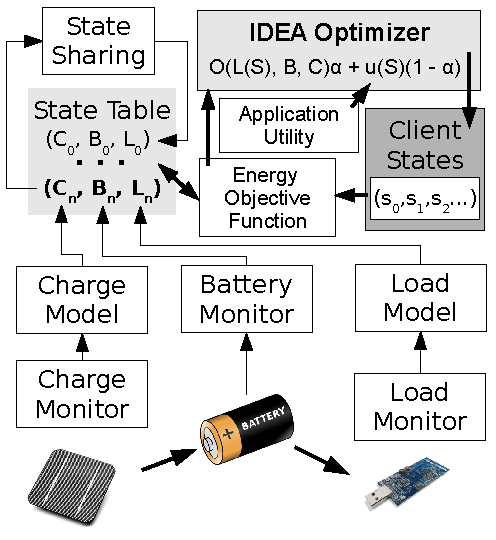
\includegraphics[width=\hsize]{./figs/IDEAArchitecture.pdf}
\end{center}

\caption{\textit{Overview of IDEA architecture.} IDEA combines load and
charge monitoring and modeling, energy data distribution, and an
application-provided energy objective function into a single service which
can easily be integrated into application components. Client states are
evaluated by the energy objective function and also assigned an application
utility. These scores are combined by the optimizer to select the state best
balancing the application's distributed energy goals against the state's
intrinsic desirability.}

\label{fig-arch}
\end{figure}

\vfill\eject
\section{Architecture}
\label{sec-architecture}

In this section, we present the IDEA architecture. Beginning with a formal
problem definition and brief overview, we then describe each major system
component in detail.

\subsection{Problem Definition}

IDEA is intended to address the problem of energy-aware tuning in sensor
network applications. In IDEA, we use the term \textit{client} to refer to
either an application (such as a tracking system) or an individual software
component (such as a MAC, routing, or time synchronization protocol) that
wishes to perform energy tuning. Clients interact with the IDEA runtime
residing on each sensor node to make decisions that impact energy consumption
and data fidelity.

Sensor network software components commonly operate by making local
decisions. For example, routing protocols~\cite{ctp,awoo-multihop} typically
form a spanning tree by each node picking a parent based on local
information, such as the radio link quality or number of hops to the sink.
Likewise, duty-cycling MAC protocols~\cite{bmac-sensys04} decide locally how
often to poll the channel and check for traffic. In IDEA, these choices are
represented as a universe of possible \textit{states} $\mathcal{S}$ that the
client can be in at any given time. As an example, a routing protocol's
states represent the set of possible parent nodes.

IDEA guides the selection of the optimal state for each client component
based on both the inherent value of that state (such as the path quality to
the sink in a routing protocol) as well as the \textit{distributed energy
impact} of choosing that state. In the case of routing, selecting a given
parent impacts the energy of the parent as well as each node along the
routing path to the sink. The ideal choice of a parent may change over time,
for example, based on network load or energy availability. IDEA clients
periodically reevaluate their current state and may switch to a new state if
it is deemed more desirable.

IDEA quantifies the distributed energy impact of each state using an
application-defined \textit{energy objective function}. Each state $s \in
\mathcal{S}$ has a corresponding a energy load vector, $\bar{L}$, where each
component $L_i^n(s_n)$ represents the estimated energy load on node $i$ that
will result from node $n$ setting its local state to $s_n$. We represent the
current battery level (in joules) at node $i$ by $B_i$ and the current
charging rate (in joules per second) at node $i$ by $C_i$. In networks
without charging capability, $C_i = 0$.

Formally, we can define the problem as follows. At a given time, let us
denote the global state of all nodes in the network as $S = \{ s_1, s_2,
\ldots, s_k \}$. The combined energy load at node $i$ induced by this
selection of states is \[ L_i(S) = \sum_{j=1}^k L_i^j(s_j) \] Based on the
current battery levels $B_i$ and charging rates $C_i$, we can define an
\textit{energy objective function} $O(\bar{L}(S), \bar{B}, \bar{C})$ that
represents the global energy impact of the global state assignment $S$.
Likewise, this state assignment has an associated application-defined
\textit{utility} $u(S)$ that represents the intrinsic desirability of the
state --- for example, minimizing path length in a routing protocol. The
choice of $u(S)$ can be provided by the application as a static function, or
learned over time by measuring application quality as it runs. IDEA is
agnostic as to its form as it is evaluated online. 

The system's goal is to determine the optimal state \[ S^\star = \arg
\max_{S} O(\bar{L}(S), \bar{B}, \bar{C}) \cdot \alpha + u(S) \cdot
(1-\alpha)\] where $\alpha$ represents the tradeoff factor between energy
impact and intrinsic utility. Setting $\alpha=1$ optimizes only for energy;
$\alpha=0$ only for application-defined utility. 

\subsection{Energy Objective Functions}
\label{subsec-energyobjectivefunctions}

Before describing the IDEA system itself, we first consider the space of
energy optimization goals that the system can target. We expect that
different applications will allocate energy differently, and the objective
function allows the behavior of IDEA to be tuned to meet a variety of needs. 

Examples of possible objective functions include:

\begin{itemize}

\item \textbf{Maximize first-node lifetime.} Depending on energy load and
availability, different nodes may run out of energy at different times. Given
the current load and charging rates, one can estimate the projected lifetime
of each node $i$ given global state $S$ as \[ \mathrm{T}(i,S) = \left\{
\begin{array}{lr} \frac{B_i}{C_i - L_i(S)} & C_i < L_i(S) \\ \infty & C_i \ge
L_i(S) \end{array} \right. \] To maximize the first-node lifetime, we find
the state $S^\star$ maximizing $O = \min_{i} T(i,S)$. This objective function
will always choose states that shift load away from the node projected to die
first, irrespective of the load that is produced on other nodes, and may be
suitable for applications whose fidelity requirements are sensitive to the
loss of single nodes.

\item \textbf{Maximize aggregate charging rate.} Given the charging rate
$C_i$, battery level $B_i$, and battery capacity $P_i$ on node $i$, the
effective charging rate given global state $S$ is \[\mathrm{A}(i,S) = \left\{
\begin{array}{lr} C_i - L_i(S) & B_i \le P_i \\ 0 & B_i = P_i \end{array}
\right. \] This reflects that when the node's battery fills it is no longer
able to collect charge. By maximizing $O = \sum_{i} \mathrm{A}(i,S)$, we
choose the state that leads to the network collecting charge as quickly as
possible. When node batteries are all still charging this objective function
will try to find the state minimizing the total system load. However, once
batteries begin to fill, it will choose states that shift load towards nodes
charging full batteries, since any additional charge these nodes capture
cannot be stored. Shifting load towards overcharging nodes allows nodes
without full batteries to charge more rapidly. This objective function
prioritizes collecting charge over preserving node uptime, and may be
well-suited to applications that expect to experience periodic charging
cycles and can tolerate some nodes running out of energy.

\end{itemize}

One of the tradeoffs IDEA objective functions may perform is between
increasing the amount of charge collected --- which leads to reducing the
cumulative network-wide impact of each IDEA component --- and periods of node
downtime resulting from poor energy distribution. Some applications may
weight node downtime differently for each node, depending on the quality of
the sensor data it is providing, its location, or other factors. Application
goals will differ, but the flexibility provided by the objective function
allows IDEA to support a variety of different requirements.

\subsection{IDEA Overview}

Thus far, we have defined the goal of the system as achieving a
\textit{globally optimal} assignment of states to each sensor node.
Performing such a global optimization would be possible through a central
node (such as the base station) collecting load and charge rates from every
node and computing the optimal assignment centrally, then informing all nodes
of their states. However, in large networks, this approach would induce large
communication overheads, reducing energy efficiency. Central control also
precludes nodes from making rapid local changes to states, for example, to
select a new parent in a routing tree if the current parent dies.

IDEA seeks to perform optimization in a \textit{decentralized} fashion, with
the goal of closely approximating the globally optimal solution. An important
observation is that \textit{most state changes only the impact energy
consumption of a node's immediate neighbors}.\footnote{In the routing case
referenced previously, while a node's choice of parent impacts all nodes
between it and the sink, it can only \textit{directly} control the load
placed on its parent. The impact on nodes farther downstream is a function of
other local choices.} Hence, nodes can perform a local optimization using
information gathered from their neighbors. Although this approach does not
ensure that the state assignment will be globally optimal, we show in
Section~\ref{sec-evaluation} that it efficiently approximates the optimal
solution.

Figure~\ref{fig-arch} provides an overview of the IDEA architecture. Each
node \textit{monitors} its own load rate, charging rate, and battery level.
Monitoring output is passed to a \textit{modeling component} that produces
models of load and charging behavior. Model parameters are distributed to
other nodes via a \textit{data sharing} component, which maintains a
distributed table allowing energy information to be queried by energy
objective functions. IDEA monitors the accuracy of each node's local model
parameters, re-propagating them as necessary to maintain the distributed
energy information.

Clients periodically evaluate their current state, which can be driven either
by application-specific behaviors (e.g., disconnection from the parent node
in the routing tree) or changes to energy availability, triggered by IDEA.
The IDEA component residing on each sensor node evaluates the energy
objective function $O$ for each possible client state, which is combined with
the client utility function $u$ to determine the next state $s'$. In the
following sections we describe each component of the architecture in more
detail.

\subsection{Monitoring and Modeling}

IDEA relies on the ability to measure and model load and charging rates at
each sensor node. This can be performed using either hardware support, as in
systems like Quanto~\cite{quanto-osdi08}, or using software monitoring, as in
Pixie~\cite{pixie-sensys08}. Modularizing these components allows IDEA to
easily support multiple node platforms and a variety of energy-harvesting
hardware.

IDEA monitors both the energy load on a node as well as the charging rate,
both represented as joules per second. The battery level is monitored as
well. The raw measurements are used to build \textit{models} that allow IDEA
to estimate the projected future energy load and availability. In addition,
the model parameters are distributed to other nodes in the network, allowing
those nodes to estimate the source node's energy load and charging profile
over time. 
\vfill\eject

IDEA provides a component that models load or charging rates by producing an
average across a fixed time window, which over time produces a
piecewise-linear model of varying load or charging rates. To estimate the
load on a single node $n$ at time $t$, $L_n(t)$, we compute $l_n =
\frac{\int_{t - \Delta t}^t \!  L_n(t)\, dt}{\Delta t}$, and distribute our
estimate $l_n$ as the single model parameter. This simple model must
distribute new parameters to incorporate time-varying load or charging rates.
However, IDEA's modeling architecture is modular and it would be
straightforward to incorporate more sophisticated charging models based on
understanding of the underlying dynamics of the energy harvesting technique
being used. A seasonal ARIMA model like that used by PRESTO~\cite{presto-TON}
would provide more accuracy when projecting future charging behavior.

IDEA distributes the battery level $B_n(t_0)$ at the time $t_0$ when it
updates the load or charging model parameters. To estimate the battery level
at time $t_1$, $B_n(t_1)$, we integrate the load and charging models, such
that $B_n(t_1) = B_n(t_0) + \int_{t_0}^{t_1} \! C_n(t) \, dt -
\int_{t_0}^{t_1} \! L_n(t) \, dt$. Integrating the simple load model is
straightforward: $\int_{t_0}^{t_1} \!  L_n \, dt = \left( t_1 - t_0 \right) *
l_n$. Other models may require more complex techniques.

We separate the modeling of load and charging rates for two reasons. First,
load and charging rates vary for different reasons: load fluctuates with
application demands, whereas charging rates fluctuate with environmental
variations. Disentangling energy inputs and outputs facilitates more accurate
modeling. Moreover, independent modeling of load and charging allows IDEA to
accurately model times when a node's battery is exhausted. While a node is
running its overall current draw $I_n = C_n - L_n$. If $I_n > \beta$, where
$\beta$ is a threshold current necessary to enable battery recharging, then
the node is charging its battery; otherwise it is discharging. Once the node
dies, however, we assume that $L_n = 0$ and $I_n = C_n$. Assuming future
energy inputs, a node that has completely drained its battery will be able to
recharge and rejoin the network once it has charged its battery past a
certain threshold.

Maintaining the accuracy of load and charging models on external nodes
requires periodically distributing updated model parameters. IDEA modeling
components monitor the accuracy of the model they have previously
distributed. Using our simple linear model as an example, if $l_n^{t_0}$ is
the model parameter distributed for node $n$ at time $t_0$, then at time
$t_1$ the model will recompute $l_n^{t_1}$. If the relative model error
$\frac{\left| l_n^{t_1} - l_n^{t_0} \right|}{l_n^{t_0}} > E$, where $E$ is an
application-configurable error tolerance, then the modeling component will
push a new parameter to the data sharing layer, which is responsible for
updating other nodes. 

\subsection{Data Sharing}

In order for nodes to make informed decisions about local state changes, they
must have knowledge of the energy profiles of other nodes. IDEA provides a
\textit{data sharing} component that distributes this information amongst
nodes in the network. The distribution service maintains a local shared data
table allowing estimated energy information for other nodes --- including
their battery levels $B_i$, load rate $L_i$, and charge rate $C_i$ --- to be
queried. Estimates are produced by evaluating the load and charging models as
described previously. Note that these values can be queried more frequently
than the underlying model parameters are updated. The use of models allows
IDEA to significantly reduce the amount of communication and energy required
to distribute this information. Of course, data sharing itself consumes
energy. However, our evaluation in Section~\ref{sec-eval} shows that this
overhead is recouped in improved overall energy efficiency. 

IDEA provides a $k$-hop data sharing component that disseminates shared data
updates using broadcast messages. This approach is similar to neighborhood
communication schemes such as Abstract Regions~\cite{regions-nsdi04} and
Hoods~\cite{hoods-mobisys}. We use a Trickle~\cite{trickle} timer to balance
rapid propagation of updates with eventual consistency in the face of link
failures. New updates cause the Trickle timer to be reset, causing immediate
data propagation. Nodes hearing the update relay it until the maximum number
of retransmissions is reached. We also utilize broadcast packets to
opportunistically retransmit data for other nodes to reduce propagation
latency. When retransmission is triggered, a node fills the broadcast packet
with other recent updates from its shared data table.

IDEA clients may piggyback on this mechanism to propagate
application-specific data to other nodes. For example, nodes may wish to
share information on MAC parameters to enable coordinated communication
scheduling. To simplify the implementation of the data sharing service we
limit the amount of space available to client applications to ensure that the
total payload fits within a single radio message.

\subsection{Client Integration}

The interface between client components and IDEA is intended to simplify
integration of IDEA with existing software. The IDEA optimizer provide
\texttt{chooseState()}, an interface that the client can invoke to select a
new state in an energy-aware fashion. Normally components may reexamine state
periodically to ensure that they respond to changes in network dynamics. IDEA
also provides event triggers that indicate when nearby energy conditions have
changed significantly, since these may also be opportunities for clients to
reevaluate their local state selection. \texttt{chooseState()} takes three
arguments:

\begin{itemize}

\item A list of possible local states $s^n = \left\{ s^n_1, s^n_2, \ldots,
s^n_k\right\}$ that the client component on node $n$ can enter;

\item For each state $s^n_i$, the intrinsic utility $u(s^n_i)$ of that state,
represented as a scalar value; and

\item For each state $s^n_i$, a projected energy load vector $\bar{L}(s^n_i)$
representing the estimated energy impact (in terms of joules/sec) induced by
the node entering state $s^n_i$. $\bar{L}$ has one element for each of the
node's neighbors.

\end{itemize}

IDEA combines this information with knowledge of energy load and availability
to determine the ideal state $s'$ the node should enter based on the weighted
combination of the objective function $O$ and the utility $u$.
\texttt{chooseState()} returns the new state $s'$ selected by the optimizer.
To reduce the possibility of two or more nodes oscillating between different
states, hysteresis can be added to the objective function to avoid wasting
energy through frequent reconfiguration.

In many cases it is straightforward to interface IDEA to existing code. As we
demonstrate in Section~\ref{sec-casestudies}, IDEA has been used to add
energy awareness to the CTP~\cite{ctp-sensys09} routing protocol with minimal
code changes. Existing software components can be supported by wrapping them
in code that estimates energy impact, enumerates states, and interfaces to
the IDEA service.

\section{Case Studies}
\label{sec-casestudies}

Throughout the rest of the paper we demonstrate IDEA using three examples.
Section~\ref{sec-evaluation} presents results demonstrating the performance
improvements that IDEA delivers for each application.

\subsection{LPL Tuning}
\label{subsec-lpltuning}

Low-power listening enables radio duty-cycling without requiring nodes
arrange fixed transmission schedules. It is well-suited for environments
where network topologies and traffic patterns are highly variable, since
these variations challenge duty-cycling techniques that assume \textit{a
priori} knowledge of traffic patterns.

When using LPL, nodes poll the radio channel at a fixed rate, listening for
packets addressed to them. The radio is shut off when not polling or sending
packets. To send a packet to another node the sender must know that node's
polling interval, and repeatedly send the packet with reduced MAC backoffs
until either the packet is acknowledged, ending the packet train and
indicating a successful transmission, or the length of the packet train
exceeds the receiver's polling interval, at which point the transmission
fails.

The choice of LPL polling rate at a given node affects the continuous energy
drain required to periodically poll the channel as well as the cost to other
nodes to communicate with the given node. Assuming we model the radio as
drawing $I_{listen}$ and $I_{transmit}$ mA of current in listen and transmit
modes, respectively, then, given an interval between radio checks of $\gamma$
sec, the current draw required to poll the channel is $\frac{1}{\gamma} \cdot
t_{check} \cdot I_{listen}$, where $t_{check}$ is the time the radio must
remain on to detect channel activity. The cost to transmit a packet to a node
using an LPL interval of $\gamma$ is, on average, $\frac{\gamma}{2} \cdot
I_{transmit}$. We can observe then that increasing $\gamma$ or polling the
channel less frequently \textit{reduces} the current draw on the receiving
node while \textit{increasing} the communication cost on sending nodes.

On the CC2420 the receive and sends costs $I_{listen}$ and $I_{trasmit}$ are
similar, and the radio can rapidly leave and return to a low-power state so
$t_{check}$ is short, on the order of 10 ms, allowing the continuous receive
cost to be minimized. As a point of comparison, using a $0.5$ second check
interval produces a current draw of 0.37 mA while requiring 4.35 mAs to send
a single packet. Put another way, sending a single packet requires as much
energy as polling the channel for over 11 seconds.

Adjusting LPL intervals offers a way of changing the energy consumption for
communication between two nodes, and an opportunity for IDEA to tune the
intervals to match the availability of energy within the network. To develop
intuition about the tuning process, we consider a simple example where Node 1
is transmitting packets to Node 2. If Node 1 has a lot of energy while Node 2
has little, then Node 2 should poll the channel slowly and let Node 1 pay the
high per-packet penalty. On the other hand, if Node 2 has a lot of energy
while Node 1 has little, then Node 2 should poll the channel rapidly,
increasing its own energy consumption but reducing the per-packet cost to
Node 1.

IDEA allows us to build a component to tune the LPL parameters on each node
adaptively. Our local state space $s_n = \left\{s_n^5, s_n^6, \ldots,
s_n^{10} \right\}$ where $s_n^j$ corresponds to polling at intervals of $2^j$
on node $n$. For each state $s^j_n$, we construct the projected energy load
vector $\bar{L}(s^j_n)$ out of two components: one measuring the receive cost
to node $n$, the other measuring the transmission cost to other nodes to send
to node $n$. The receive cost on node $n$, $\bar{r}_n$, has only a single
component for node $n$, $r_n^n(s_n^j) = \frac{1024}{2^j} \cdot 0.010
\textrm{sec} \cdot 19.7$ mA, where $0.010$ sec is the check interval and
$19.7$ mA is the radio receive current. The transmission cost to nodes
sending to node $n$, $\bar{t}_n$, has components of the form $t^i_n(s_n^j) =
\frac{1}{2} \cdot \frac{2^j}{1024} \textrm{sec} \cdot \delta(i,n) \cdot 17.4$
mA, where $\delta(i,n)$ is the rate at which node $i$ is sending packets to
node $n$ and $17.4$ mA is the radio transmission current. We construct the
total energy load vector $\bar{L}_n(s^j_n)$ as the component-wise sum of
$\bar{r}_n$ and $\bar{t}_n$, and pass this information to IDEA to evaluate
each state.

When the LPL tuning component switches states, it must propagate this
information to nearby nodes that might be sending it data. We use the ability
of IDEA to propagate component state to disseminate this information. The
tuning component intercepts outgoing transmissions, queries IDEA for the
correct LPL interval to use for the given destination, and sets the packet's
LPL interval accordingly.

Changing the LPL interval also effects the total throughput possible over the
link, which provides the component-specific measure of desirability, although
the relationship is complicated by the ability of LPL to bunch transmissions
to amortize the cost of awakening the receiver. For our evaluation we chose
to set the tradeoff factor $\alpha=1$ and optimize only for energy, since the
throughput of the link was not a limiting factor at the data rates we tested.

Finally, low-power probing (LPP) approaches available in
Contiki~\cite{contiki} and made possible by BackCast~\cite{backcast-hotnets}
improve on the LPL approach by using receiver-initiated probing to eliminate
the high channel contention caused by LPL's packet trains. However, they
produce similar energy consumption patterns to LPL and could be tuned in the
same way. We have focused on tuning LPL parameters due to LPL's availability
in the standard TinyOS distribution, but are exploring LPP-based approaches
as future work.

\subsection{Energy-Aware Routing}
\label{subsec-ictpcasestudy}

The second example shows how to integrate IDEA with an existing routing
protocol, namely the Collection Tree Protocol (CTP)~\cite{ctp-sensys09}. CTP
is a spanning-tree routing protocol that is a standard component in
TinyOS~\cite{tinyos-asplos00}. In CTP, each node selects its parent in the
spanning tree based on the \textit{expected number of transmissions} (ETX) to
reach the sink. This is an additive metric intended to limit queue occupancy
at nodes along each routing path and maximize packet delivery rates. Although
ETX can be directly converted to an energy measure (assuming the energy costs
to transmit along a link are known), CTP does not explicitly consider energy
availability in its routing decisions.

We integrate IDEA with CTP to create \textit{ICTP}, an energy-aware
load-balancing routing protocol that combines the use of ETX with IDEA's
energy objective function. As described in
Section~\ref{subsec-energyobjectivefunctions}, we parameterize the tradeoff
between pure ETX and pure energy objective using the weighting factor
$\alpha$. When $\alpha = 1$ the minimum ETX path is always used and ICTP
behaves identically to unmodified CTP. When $0 < \alpha < 1$, potential
parents with path ETX $<$ minimum ETX $\cdot \frac{1}{\alpha}$ will be
considered, with the one producing the best energy objective score chosen.
When $\alpha = 0$, ETX is not considered at all and parent selection is
performed entirely on the basis of energy. Hence, $\alpha$ indirectly
controls the degree of path stretch that is induced by energy awareness. 

\vfill\eject

In order to build routes, CTP must periodically broadcast the current parent
and ETX to neighboring nodes. ICTP adds additional information to these
broadcasts, specifically the \textit{expected power}, or \textit{EPX}, for
transmissions to the node's parent. This information increases the size of
the broadcast packet sent by ICTP slightly, but does not appreciably affect
the energy consumption of the protocol's own data sharing, since the cost to
transmit a packet using LPL is a function of the receiver's polling interval,
not the packet size.

The local state space $s_n = \left\{s_n^{p_1}, s_n^{p_2}, \ldots, s_n^{p_k}
\right\}$ is defined by the node $n$'s neighbors $p_n = \left\{p^1, p^2,
\ldots, p^k \right\}$, each of them a prospective parent. CTP uses four-bit
wireless link estimation~\cite{Fonseca07} to estimate the ETX to each
neighbor, which ICTP multiplies by the power-per transmission to produce the
EPX to each neighbor, $EPX(n, p_n^i)$. Through ICTP data dissemination node
$n$ also learns the EPX from each neighbor to their current parent,
$EPX(p_n^i, \textrm{parent}(p_n^i))$. We have modified CTP to measure the
traffic rate $\delta(n)$, which is the number of packets per given interval
that node $n$ is forwarding to the sink. This is a function of both its own
packet generation rate and of the traffic induced by nodes upstream that it
is routing for. Given these parameters the projected energy load vector
$\bar{L}(s_n^{p_i})$ has two components: $L_n = \textrm{EPX}(n, p_n^i) \cdot
\delta(n)$ and $L_{p_i} = \textrm{EPX}(p_n^i, \textrm{parent}(p_n^i)) \cdot
\delta(n)$. Based on this information, IDEA chooses the best neighbor as the
node's parent.

Depending on the energy objective function chosen ICTP responds to variations
in load and charging rates in different ways. For the following discussion we
assume that the application uses the \textit{maximize first-node lifetime}
objective function described in
Section~\ref{subsec-energyobjectivefunctions}, and so is willing to trade off
reduced charging rates or lifetimes at nodes that are not the network's
lifetime bottleneck in order to increase the lifetime of the node projected
to die first. Routing trees by their very nature concentrate load near the
base station, which we assume is powered. Without considering variances in
non-routing load or charging rates ICTP will attempt to balance load across
nodes that can communicate directly with the base station, arranging the
routing tree considering both the number of nodes upstream from each of the
base station's neighbors and the quality of their link to the base station.

ICTP also responds to spatial variations in charging rates by building a tree
that is sensitive to where in the network energy is available. ICTP will
route around shadows in the network, or build routing backbones using
quickly-charging nodes or nodes whose batteries are full while attempting to
push nodes low on batteries into leaf roles, reducing or eliminating their
routing responsibilities.

Because ICTP reacts to changes in energy available by potentially choosing
routes with larger ETX, small values of $\alpha$ can begin to effect the
achieved packet delivery rate. We were able to find values of $\alpha$ that
produced significant performance improvements while leaving the delivery rate
unaltered. CTP has a persistent retransmission policy which assists us in
achieving good performance.

\subsection{Distributed Localization}

The third case study illustrates how to use IDEA to control discrete, rather
than continuous, network behavior. We consider a system designed to perform
acoustic source localization. Several previous systems have explored this
application in different contexts, including urban sniper
localization~\cite{shooter-localization} and localizing animals based on
mating calls~\cite{girod-marmots}. Using IDEA, it is possible to carefully
manage the energy load at each sensor node to prolong battery lifetime while
maintaining high localization accuracy.

Acoustic source localization involves calculating the location of an acoustic
source by collecting arrival times at several stations and performing a
back-azimuth computation. We assume a dense sensor network deployment, so
that an acoustic event is detected by many sensors. We also assume that for
each event, any set of four sensors that heard the event can correctly
perform the localization to within the application's error tolerance. 

A centralized approach to localization requires nodes to transmit data to a
base station where the computation is performed. Because we assume that nodes
cannot accurately compute an arrival time by only considering their own
sampled data, they must transmit a sizeable amount of data to the base
station to implement the centralized strategy, with the bulk data transfer
required producing a significant load on the nodes that heard the event as
well as nodes required to route data. This approach also does not scale well
as the size of the network increases.

To avoid the overheads of centralization we want to perform the localization
inside the network. However, the cost to transmit signals and perform the
computation are still high, so it is important that localization be done in a
way sensitive to the availability of energy within the network.

When an event occurs, the goal is to select a single \textit{aggregator} node
and three \textit{signal provider} nodes from the set of nodes that detected
the event. The signal providers will transmit a portion of the acoustic
signal to the aggregator, which performs the localization computation using a
time-of-arrival and angle-of-arrival computation~\cite{Niculescu03adhoc}.
For each event we expect multiple valid aggregator and signal provider sets
to exist, each with its own energy consumption signature. We refer to a
selection of four such nodes as a \textit{localization plan}. 

Nodes that heard the signal participate in a leader election process, seeded
by the value of the IDEA energy objective function for each proposed
localization plan. Each candidate aggregator computes the energy objective
function for the localization plan or plans that they are the aggregator for.
If more than three nodes within a single hop of an aggregator heard the
event, then the aggregator will have multiple plans to consider. The
aggregator chooses the local plan with the best score and broadcasts a
message advertising that score, which is propagated to all nodes that heard
the event. If the aggregator does not hear a broadcast with a better score,
it assumes that it won the leader election and proceeds to perform the
localization as planned. 

\section{Evaluation}
\label{sec-evaluation}
\label{sec-eval}

To evaluate IDEA, we build and test the two energy-aware components and one
energy-aware application described in Section~\ref{sec-casestudies}. For the
LPL tuning and routing components, we compare the performance of our
IDEA-based implementations to approaches that are not energy-aware. For the
third application, we use IDEA to implement several energy objective
functions and compare their performance against each other and against a
heuristic that does not consider energy availability.

\vfill\eject

\subsection{Experimental Setup}
\label{subsec-experimentalsetup}

Throughout the evaluation we present results run in several different
environments. We have implemented IDEA for TinyOS in order to run experiments
on MoteLab~\cite{motelab}, our 180~node wireless sensor network testbed. We
also present results obtained using TOSSIM~\cite{tossim}, the TinyOS
simulator. TOSSIM incorporates a closest-fit pattern matching noise model to
accurately capture complex link dynamics~\cite{cpm-ipsn07}. TOSSIM allows us
to run longer experiments incorporating various solar charging models. To
improve the realism of TOSSIM we began with a modified version developed for
the Koala project~\cite{koala-ipsn08} and performed further modifications to
correctly simulate the operation of LPL. We use information collected on
MoteLab to build a realistic TOSSIM radio model for our simulations. Finally,
for the third application we built a Python simulator to allow rapid
prototyping of various energy objective functions.

IDEA is designed to tune components in the face of variations in both load
and charging rates, and to test this we present experiments using solar
charging data collected off of a solar panel deployed on an Arlington, MA
rooftop in March, 2009. Battery levels are calculated using a charging model
based on a Nickel-Metal Hydride battery technology with a 66\% charging
efficiency. We attenuate this data to simulate the charging produced by solar
panels of several different sizes in order to evaluate IDEA's performance as
available energy changes. We also perform experiments with a randomly
attenuated charging profile to simulate bad solar panel placement or
obstacles to incident sunlight effecting the spatial distribution of
collected energy.

For our MoteLab experiments we determine the system's ability to span periods
without charging inputs. We use two sets of initial conditions based on the
interaction between the charging data we collected and the capacity of the
batteries deployed. If the solar panel is large enough it will provide
considerable charging input and completely charge small batteries during the
day, so that all nodes begin the night with full batteries. If the solar
panel is not large enough to completely charge the batteries nodes will begin
the night with varying amounts of charge depending on their load rates during
the day.

Energy tracking is done by IDEA using a software-only approach developed for
the Pixie~\cite{pixie-sensys08} project. The component captures state
transitions and applies an energy consumption model for each state based on
current consumption measured offline. In the future we would like to
integrate a more accurate hardware-driven approach such as
iCount~\cite{icount-spots08}. The short lifetimes for some experiments are
explained by the use of extremely small batteries, which were chosen to allow
experiments to complete in reasonable amounts of time. We expect that
application developers will want to use a battery size and charging
technology suitable to allow their system to achieve a desired level of
performance, and the improvements in energy efficiency possible using IDEA
will allow smaller batteries or solar panels to be used, reducing the size
and cost of the hardware package.

Experiments for the LPL tuning and energy-aware routing cases use the
first-node death energy objective function described in
Section~\ref{subsec-energyobjectivefunctions}, and therefore we evaluate the
network lifetime as the time at which the first node runs out of energy. Our
distributed localization application illustrates the process of designing an
effective energy objective function when the overall goal of the system is
known.

\subsection{LPL Parameter Tuning}
\label{subsec-lplparametertuning}

\begin{table}[t]
\begin{center}
\begin{tabular}{|l|ccc|}
\hline
\textbf{Initial Battery} & \multicolumn{2}{c}{\textbf{Lifetime (hours)}} & \textbf{Increase} \\
\textbf{Levels} & \textbf{Static} & \textbf{Tuned} & \textbf{(\%)} \\ \hline
Uniform & 4.6 & 5.6 & 22\% \\
Random & 2.8 & 3.0 & 7\% \\ \hline
\end{tabular}
\end{center}

\caption{\textit{LPL tuning performance on MoteLab.} The table shows results
for MoteLab experiments comparing the performance of the IDEA-driven LPL
tuning component against the best static parameter solution. IDEA shows gains
for both the case where all nodes start with the same battery level and
randomly initialized battery states.}

\label{table-lplvoptimalmotelab}
\end{table}

We begin by evaluating the IDEA-driven LPL parameter tuning component
described in Section~\ref{subsec-lpltuning}.
Figure~\ref{table-lplvoptimalmotelab} summarizes the results of experiments
conducted on a 20~node subset of the MoteLab sensor network testbed. We
configure the nodes into a collection tree with each node sending messages to
the sink once every 2 minutes. As a point of comparison we ran experiments
using static intervals assigned a priori, with all nodes using the same LPL
interval. We compared the results from all six intervals and picked the one
that performed the best. Note that this experimentation itself is a form of
tuning and would be difficult to do beforehand. We ran one hour testbed
experiments and used each node's rate of energy consumption to compute a
projected lifetime.

The table shows that the tuned LPL intervals produce improvements in
projected lifetimes when compared with the best static interval under both
non-charging scenarios discussed in Section~\ref{subsec-experimentalsetup}.
We observe an improvement of 22\% for the case where nodes start with the
same initial charge and 7\% when random initial battery levels are used. This
is despite the fact that the LPL tuning component produces significant
overhead propagating new state early in the experiment as nodes are moving
from their initial states into their IDEA-tuned intervals.

\begin{table*}[t]
\begin{center}
\begin{tabular}{|l|cccc|}
\hline
\textbf{Solar Charging} & \multicolumn{3}{c}{\textbf{Lifetime (hours)}} &
\textbf{Increase} \\
\textbf{Pattern} & \textbf{Static} & \textbf{Tuned} & \textbf{No Overhead} & \textbf{(\%)} \\ \hline
Large Panel & 22.7 & 23.8 & 24.0 & 5\% \\
Small Panel & 16.8 & 18.9 & 21.2 & 13\% \\
Randomly & \multirow{2}{*}{13.8} & \multirow{2}{*}{18.6} & \multirow{2}{*}{20.4} & \multirow{2}{*}{35\%} \\
Attenuated & & & & \\ \hline
\end{tabular}
\end{center}

\caption{\textit{LPL tuning performance with solar charging.} This table
displays results for TOSSIM experiments comparing IDEA-based LPL parameter
tuning with the best static interval and an overhead-free version of IDEA.
IDEA shows gains over the non-tuned approaches across a range of different
solar charging profiles.}

\label{table-lplvoptimaltossim}
\end{table*}

Figure~\ref{table-lplvoptimaltossim} summarizes results from experiments
performed on TOSSIM that include solar charging inputs discussed above. IDEA
provides 5\% and 10\% performance improvements for cases in which all nodes
see the same input charging profile and a 35\% improvement in the case where
charging inputs are randomly attenuated. We believe that this is due to the
increased difference in battery levels due to the random attenuation, which
creates more diversity in the amount of available charge. The table also
shows numbers that indicate the best that IDEA can do when its overhead is
artificially eliminated, showing that future work on improving the load and
charge modeling and more efficient data sharing will continue to improve
performance.

\begin{figure}[t]
\begin{center}
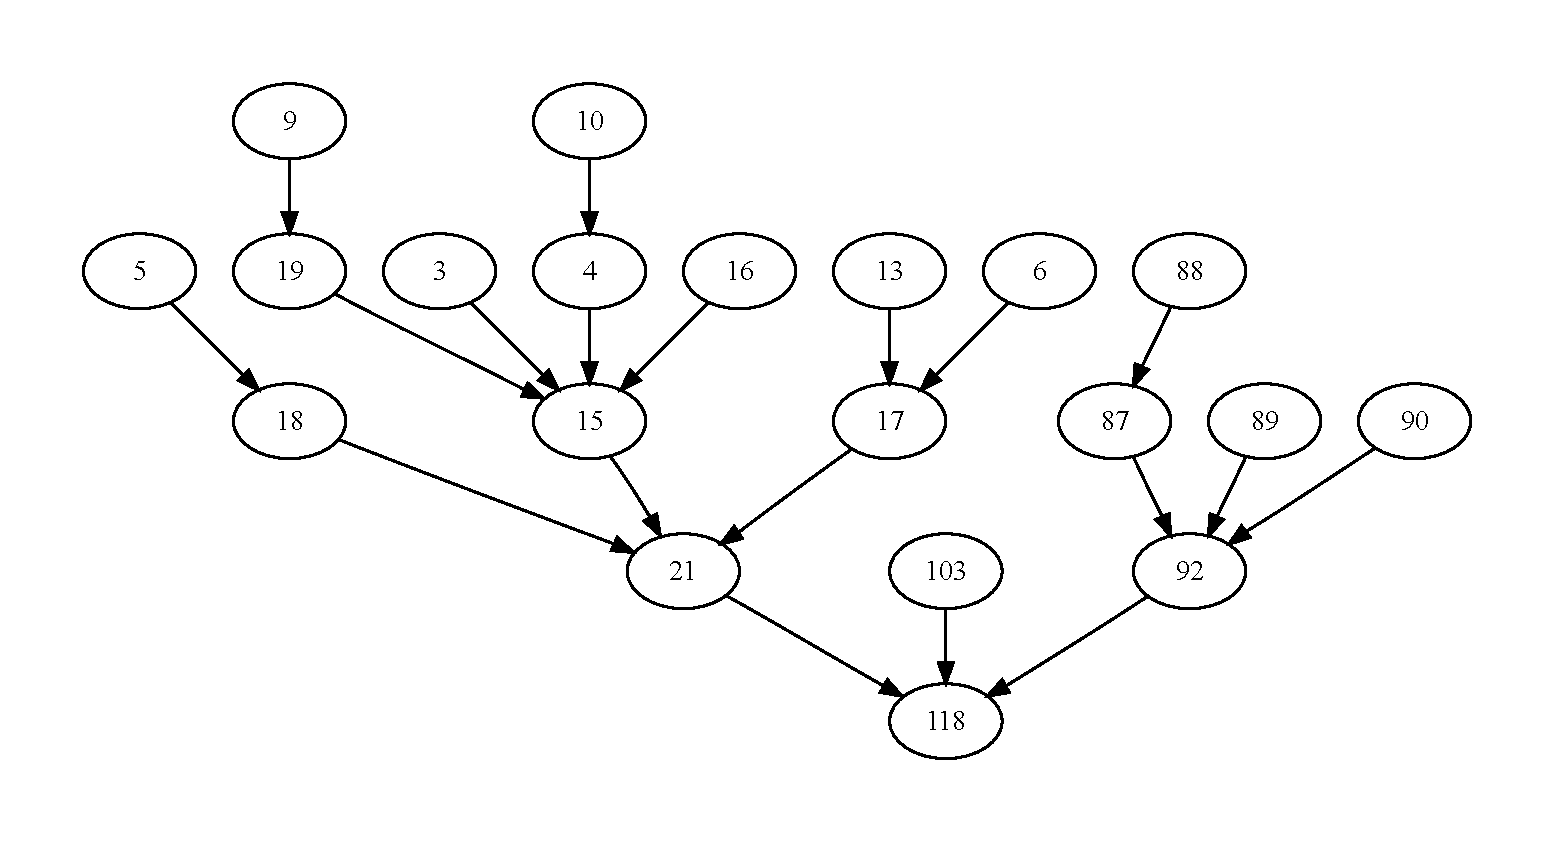
\includegraphics[width=\hsize]{./figs/lpltune_topology.pdf}
\end{center}
\caption{\textit{Topology used for LPL tuning experiments.}}
\label{fig-lpltopology}
\end{figure}

\begin{figure}[t]
\begin{center}
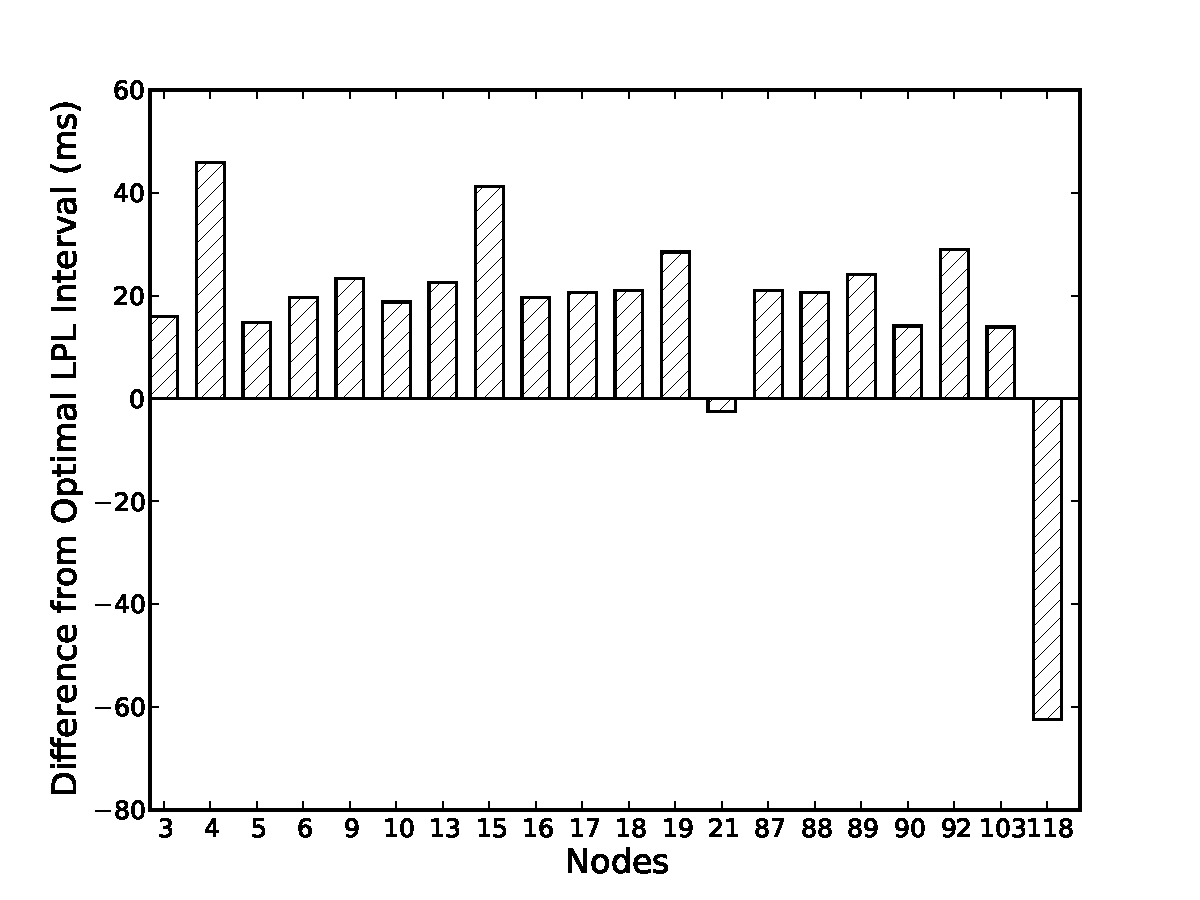
\includegraphics[width=\hsize]{./figs/graph_lpl_interval_comparison.pdf}
\end{center}

\caption{\textit{LPL interval comparison with optimal.} To assess the degree
to which the IDEA-driven approach finds a near optimal global state we plot
the percent difference between the intervals chosen by the IDEA-tuned and
offline optimal systems. The plot demonstrates that IDEA sets the LPL
intervals of nodes similarly to the optimal solution and helps explain its
performance.}

\label{fig-intervalvoptimal}
\end{figure}

In the non-charging case we can produce an offline-optimal estimate of the
possible performance by treating the problem as a multi-dimensional,
multiple-choice knapsack problem and computing a solution. We use the optimal
solution as a qualitative point of comparison in
Figure~\ref{fig-intervalvoptimal}, which shows the differences between
intervals picked by the IDEA-driven and optimal solutions for a non-charging
TOSSIM experiment using a 20~node tree, shown in
Figure~\ref{fig-lpltopology}. Most nodes are leaf nodes and IDEA correctly
choose the maximum interval possible. IDEA chooses near-optimal intervals for
Node 21, the energy bottleneck (within 1\% of optimal) and the worst-case,
Node 118 (the sink), was still within 15\% of optimal.

\begin{figure}[t]
\begin{center}
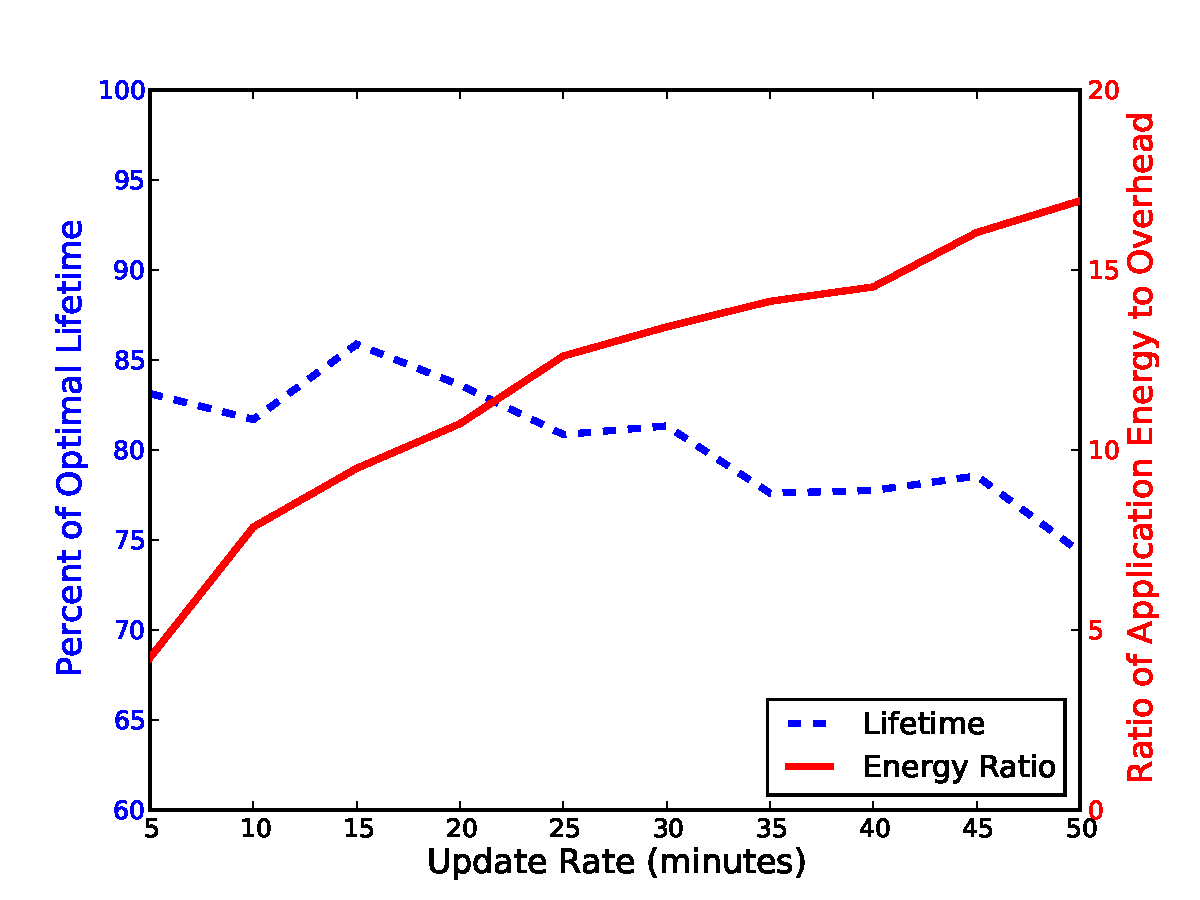
\includegraphics[width=\hsize]{./figs/graph_update_rate_overhead.pdf}
\end{center}

\caption{\textit{Optimality and overhead.} IDEA consumes energy in order to
propagate load, charge, and state information. For the LPL-tuning component
the energy overhead is related to the rate at which we re-tune the local LPL
interval, load model, and charge model. This plot shows both the IDEA
overhead and the degree of optimality achieved as the update rate is varied.}

\label{fig-lploverhead}
\end{figure}

We also use the optimal results to examine the impact of the overhead of the
IDEA LPL-tuning component as we vary the rate at which updates are performed
in the system. IDEA can vary how often nodes evaluate their LPL intervals as
well has how often to evaluate load and model parameters. A more frequent
evaluation of LPL intervals allows the system to more quickly react to
changes in the network with the potential of higher energy costs as more
state changes may need to be propagated across the network. By the same
token, more frequent evaluation of load and charge model parameters allow
IDEA to quickly react to fluctuations in energy in the network, but may
result in more energy consumed as new models must be propagated via the data
sharing mechanism.

\vfill\eject

Figure~\ref{fig-lploverhead} shows the variation in lifetime, plotted as
percent of the optimal solution, and the percent overhead used by IDEA
overall, as well as the subset of IDEA energy used for tuning the LPL
parameters as we vary both the LPL and load model evaluation rate. 

As we decrease the update rate, model parameters are shared less frequently
and the network consumes less energy, causing the overhead to decrease. LPL
tuning overhead remains relativity constant as the workload for this
application is static and most evaluation periods do not produce a change in
LPL intervals. For this application the lifetime curve shows the best results
with an update rate of 15 minutes. At the left end of the curve with a rapid
update rate the overheads associated with data sharing reduce the systems
lifetime, and at the right end of the curve the system is slower to find the
optimal state and may spend some time with sub-optimal intervals and the
lifetime again suffers. Across the entire range, however, the achieved
network lifetime remains above 74\% of the optimal offline solution.

\vfill\eject

\subsection{ICTP: Energy-Aware Routing}

\begin{figure}[t]
\begin{center}
\textbf{(a)}\\
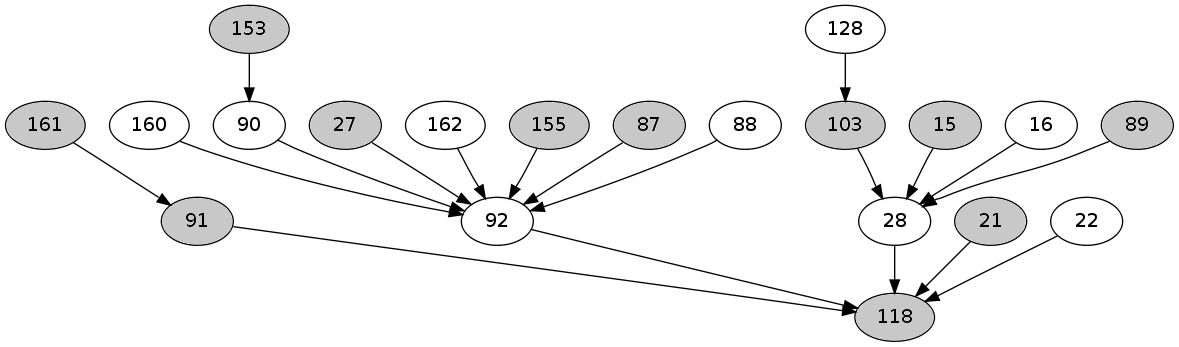
\includegraphics[width=\hsize]{./figs/STOCK.png}\\
\textbf{(b)}\\
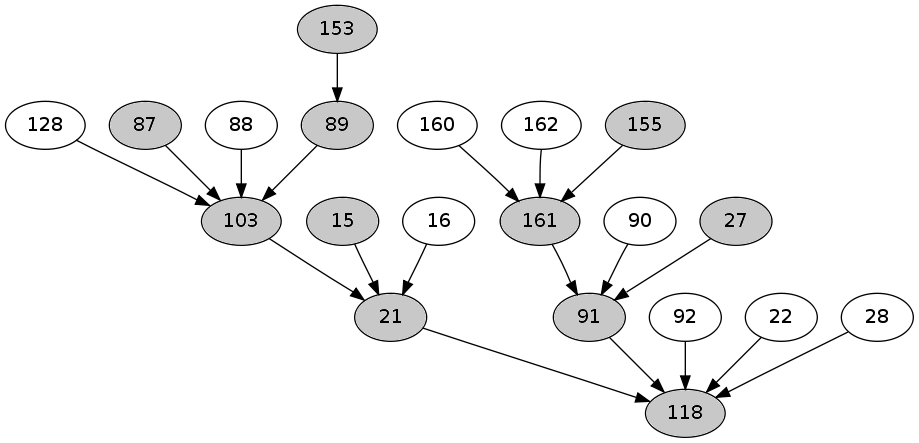
\includegraphics[width=\hsize]{./figs/ICTP.png}\\
\end{center}

\caption{\textit{Qualitative comparison of stock CTP and ICTP.} For this
experiment odd-numbered nodes (shaded) were set to charging rapidly, while
even-numbered nodes were not charging. Unmodified CTP builds the tree shown
in (a), which routes many packets through the even nodes. ICTP builds the
tree shown in (b), which moves all even nodes to leaf roles.}

\label{fig-ictpqualitative}
\end{figure}

Using IDEA we were able to integrate energy awareness into CTP, the routing
protocol included as part of TinyOS. For these experiments each node in a
20~node network is sending packets to the sink at the rate of 6 packets per
second. Static LPL intervals of 0.5 second were used. 

Figure~\ref{fig-ictpqualitative} shows a qualitative demonstration of the
differences between energy-aware and non-energy-aware routing trees. This
TOSSIM simulation ran with all odd numbered nodes charging rapidly and all
even numbered nodes not charging (with the exception of the sink, Node 118,
which we assume is powered). While this is an unrealistic charging pattern,
it produces a clear difference in the routing protocol behavior.
Figure~\ref{fig-ictpqualitative}(a) shows that unmodified CTP is unaware of
these charging differences and puts several even nodes, such as Node 92, into
positions where they are routing for multiple nodes. The total number of
nodes upstream from even numbered nodes in the stock CTP case is 14. In
contrast, ICTP realizes that the odd-numbered nodes have energy to spare and
the even-numbered nodes are lacking, and moves all even nodes to leaf roles.
None of the even nodes in Figure~\ref{fig-ictpqualitative} are routing data.

Using a setup similar to that described in
Section~\ref{subsec-lplparametertuning}, we compared the performance of ICTP
to unmodified CTP using 24-hour TOSSIM simulations and the three different
solar charging scenarios previously described. As
Table~\ref{table-lplvoptimaltossim} shows, ICTP shows improvements in
lifetime over stock CTP of between 11 and 27\%. The different routing trees
formed by ICTP did not effect the packet delivery rates appreciably with the
largest change in packet delivery rate being 2.8\% (97.8\% for CTP vs. 95.0\%
for ICTP).

Finally, Table~\ref{table-etxsearchradius} shows how IDEA can trade off
application utility with the energy objective function. The simulation
experiment uses a 25~node grid topology and, similar to the previous
experiment, half the nodes are charging rapidly while the other half are not.
Here our application-defined metric is expected transmissions to reach the
sink (ETX). A purely ETX-based tree will use the shortest route without
routing around the uncharging nodes, whereas an energy-aware tree will avoid
the uncharging nodes by constructing longer routes. We expect that,
prioritizing ETX will cause the total ETX of the entire tree --- defined as
the sum of the ETX of all the routes in use --- to decrease, while
prioritizing energy performance will cause the first-node lifetime of the
tree to increase.

Indeed, Table~\ref{table-etxsearchradius} confirms this is the case. For each
experiment, we restrict the set of acceptable parents to be the minimum
available parent ETX plus an extra amount we call the ETX search
margin. For example, if the minimum available parent ETX is 5 and the ETX
search margin is 10, then we will consider all parents with ETX < 15. As the
search margin increases, IDEA will examine longer routes that may provide
better energy performance. As the table shows, increasing the ETX search
margin leads to longer average routes but also improves overall network
lifetime.

\begin{table}[t]
\begin{center}
\begin{tabular}{|l|ccc|}
\hline
\textbf{Solar Charging} & \multicolumn{2}{c}{\textbf{Lifetime (hours)}} & \textbf{Increase} \\
\textbf{Pattern} & \textbf{CTP} & \textbf{ICTP} & \textbf{(\%)} \\ \hline
Large Panel & 17.1 & 19.0 & 11\% \\
Small Panel & 10.5 & 13.3 & 27\% \\
Random Attenuation & 10.5 & 12.2 & 16\% \\ \hline
\end{tabular}
\end{center}

\caption{\textit{ICTP performance with solar charging.} The table summarizes
the improvements in performance obtained by replacing CTP with ICTP. Three
different solar charging profiles are used corresponding to a large panel
that completely charges all batteries during the day, a small panel that does
not completely charge all batteries during the day, and a randomly attenuated
charging profile that varies node-to-node.}

\label{table-ictpvoptimaltossim}
\end{table}

\begin{table}[t]
\begin{center}
\begin{tabular}{|l|cc|}
\hline
\textbf{ETX Search} & \textbf{Total ETX} & \textbf{Network Lifetime} \\
\textbf{Margin (ETX)} & \textbf{(ETX)} & \textbf{(sec)} \\ \hline
0 & 2442 & 4357 \\
10 & 2591 & 4737 \\
20 & 3207 & 5116 \\
50 & 3127 & 6216 \\
100 & 3442 & 6502 \\ \hline
\end{tabular}
\end{center}

\caption{\textit{Tradeoff between energy-awareness and application utility.}
The table shows results illustrating how IDEA can parameterize the tradeoff
between optimizing for application-defined utility and the energy objective
function.}

\label{table-etxsearchradius}
\end{table}

\subsection{Distributed Localization}

To evaluate the distributed localization application we built a Python
simulator, which improves significantly on TOSSIM performance at this scale
and allowed rapid iteration and experimentation with different energy
objective functions. Our simulator models acoustic event sources within the
sensor network, each of which triggers a distributed localization operation.
The energy overheads of communication, both the leader election process and
the subsequent data transfer, are modeled in the simulator based on empirical
measurements taken on our MoteLab testbed.

\begin{figure*}[t]
\begin{center}
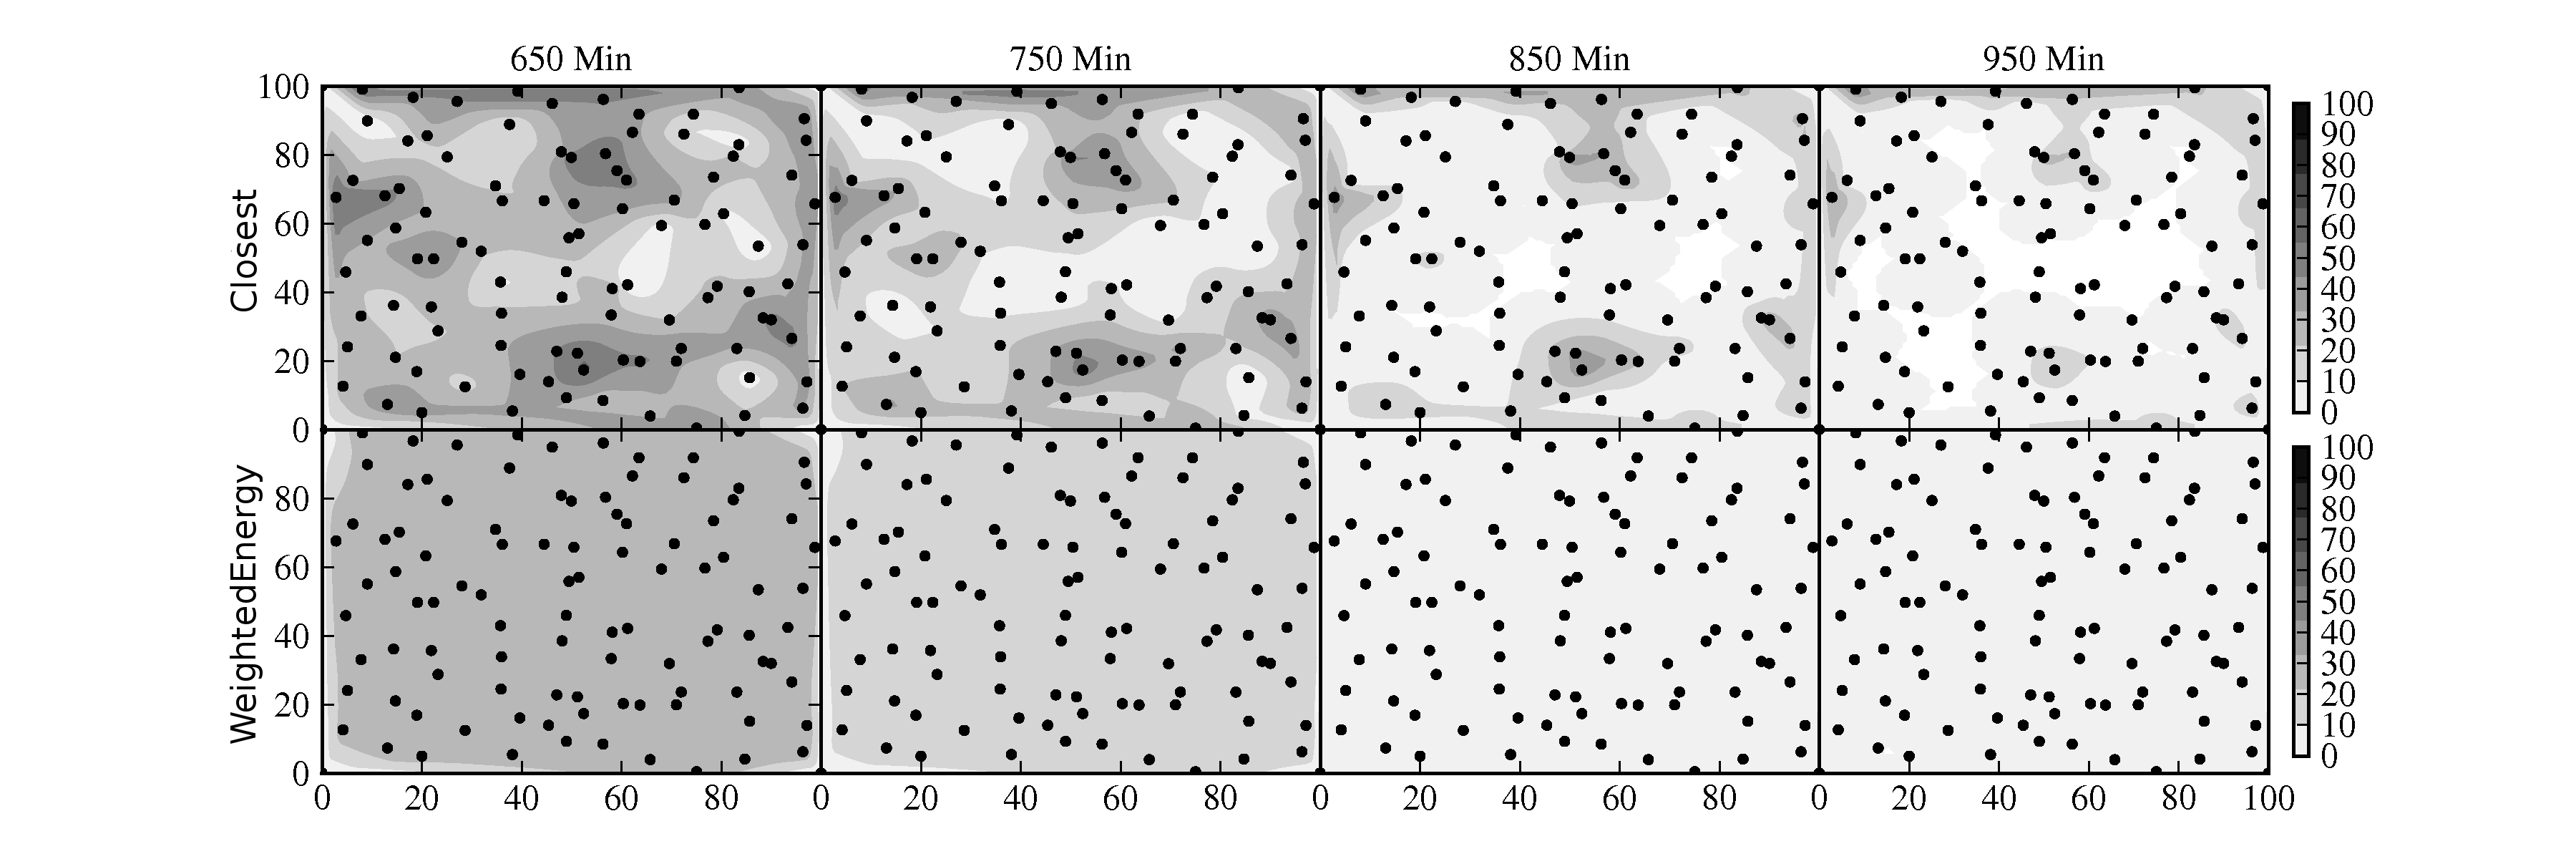
\includegraphics[width=\hsize]{./figs/graph_density_vs_time0406_2151.png}
\end{center}

\caption{\textit{Energy density over time.} Energy densities for the
\texttt{Closest} heuristic and IDEA using the \texttt{WeightedEnergy}
objective function are shown at four points in time. The event distribution
is uniform. IDEA enables better load distribution, which leads to a longer
application lifetime.}

\label{fig-localizationdensityvtime}
\end{figure*}

For these experiments we arranged 100 nodes into a 100~m by 100~m area,
resulting in the placements shown in
Figure~\ref{fig-localizationdensityvtime}. We simulate a sensing range equal
to the communication range, each set to 20~m, and randomize the reliable
transfer protocol bandwidth across each link to between 768 and
1280~bytes/sec, a feasible range based on results from data transfer
protocols such as Flush~\cite{flush-sensys07} and
Fetch~\cite{volcano-osdi06}. Events are simulated using a uniform random
distribution so that events have equal probability of occurring anywhere in
the sensor field.

To evaluate network performance, we define \textit{capability} of the network
as the percent of the last 100 operations that succeeded, where success is
defined as localizing the event. We assume that the application requires that
the network be able to localize 90\% of events that occur, and design our
energy objective functions with this in mind. We quote the system lifetime as
the the 90\% capability time, that is the time at which the network's
capability drops below 90\%.

We experimented with several approaches to choosing a localization plan, one
that does not use IDEA and three that do using different energy objective
functions:

\begin{enumerate}

\item \textbf{\texttt{Closest}:} produces a localization plan with the node
closest to the event source as the aggregator and the next three closest
nodes as signal providers. We assume a real solution would use an imperfect
estimate of proximity such as total signal energy or signal-to-noise ratio,
but for the simulations we use the known simulated event location to choose
the closest nodes. \texttt{Closest} does not require energy state information
and so could be implemented without IDEA. It is implemented as an example of
a plausible non-energy-aware solution.

\item \textbf{\texttt{MaxEnergy}:} chooses the node with the most energy
(that heard the event) as aggregator and the next three highest-energy nodes
as signal providers.

\item \textbf{\texttt{TotalEnergy}:} chooses the localization plan that
consumes the lowest amount of total energy summed across all nodes in the
network.

\item \textbf{\texttt{WeightedEnergy}:} weights the total energy consumption
using a similarity metric derived from the cosine similarity index to measure
the degree to which the energy vector for the localization plan is a good
``fit'' given the current energy availability.

\end{enumerate}

\begin{figure}[t]
\begin{center}
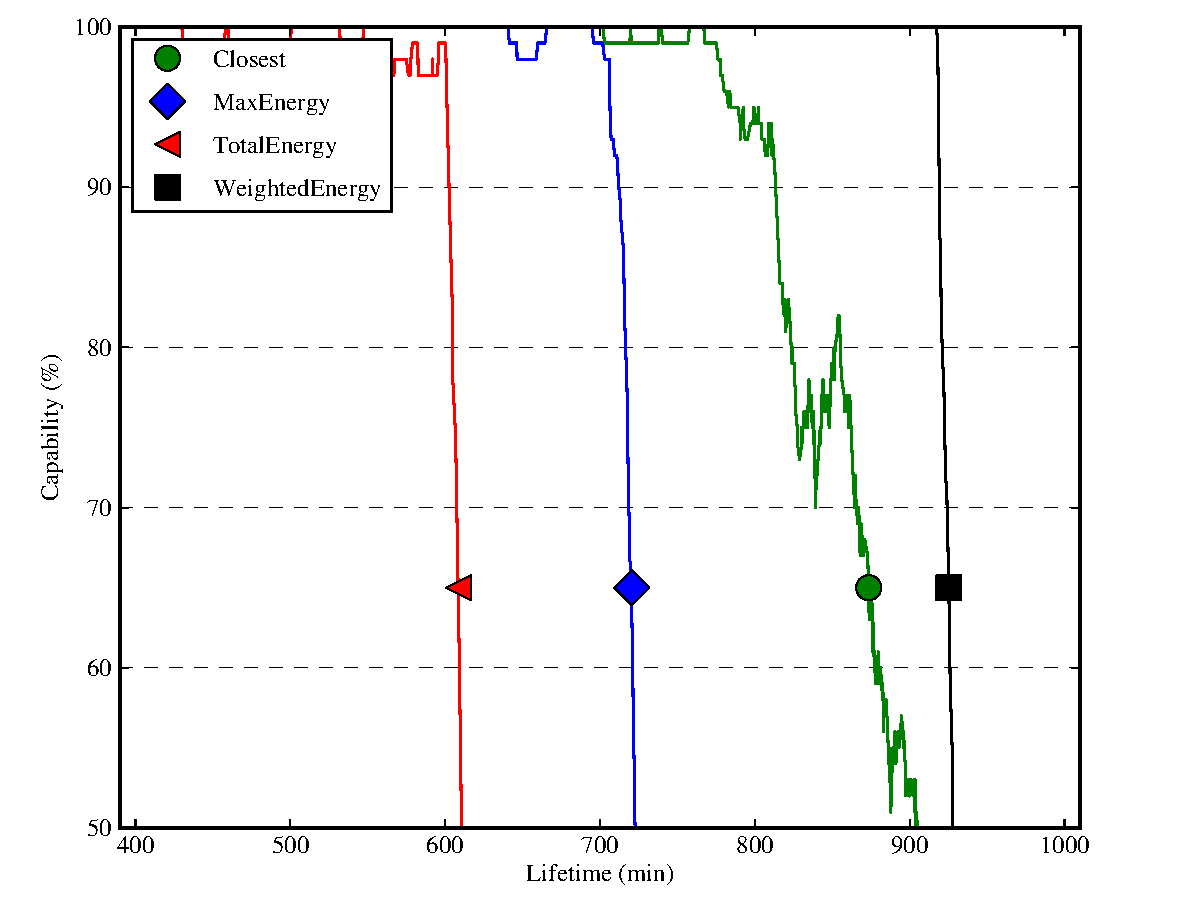
\includegraphics[width=\hsize]{./figs/graph_capability_vs_time1210_2100.pdf}
\end{center}

\caption{\textit{Performance of IDEA objective functions and heuristic.}
Simulation results are shown for the localization application. The graph
compares the \texttt{Closest} heuristic, implemented without using IDEA,
against three different IDEA objective functions: \texttt{MaxEnergy},
\texttt{TotalEnergy} and \texttt{WeightedEnergy}. The \texttt{WeightedEnergy}
approach using IDEA outperforms the non-energy-aware approach while the other
objective functions perform more poorly.}

\label{fig-ideavsheuristics}
\end{figure}

\vfill\eject

We began by experimenting with the \texttt{Closest}, \texttt{MaxEnergy} and
\texttt{TotalEnergy} approaches. As Figure~\ref{fig-ideavsheuristics} shows,
the \texttt{Closest} heuristic outperformed the two IDEA-based approaches.
However, when examining the energy density plot shown in
Figure~\ref{fig-localizationdensityvtime} for the \texttt{Closest} heuristic
we could see that it led to concentrations of available energy on nodes at
dense locations on the irregular grid. This is despite the uniform
distribution of acoustic event sources, which one might expect to produce
good energy load distribution without the need for tuning. After exploring
several additional approaches we found an energy objective function capable
of producing extremely good load distribution, the \texttt{WeightedEnergy}
approach described above. Figure~\ref{fig-ideavsheuristics} shows that it
outperforms \texttt{Closest}, increasing the network's lifetime by 15\%,
while Figure~\ref{fig-localizationdensityvtime} illustrates how it utilizes
all the nodes' available energy. Our experience with the localization
application illustrates the role of the proper energy objective function in
enabling good application performance, and points to the increases in system
lifetime possible through better energy distribution. 

\section{Related Work}
\label{sec-related}

Previous work has addressed the problem of energy load balancing in contexts
such as sensor coverage, role assignment, and energy-aware routing. Other
efforts in sensor networks have focused on reducing the power consumption at
individual nodes without considering energy distribution. Many of these
efforts are specific to a particular application or component and do not
provide a service like IDEA that can be used by a variety of applications. 

A number of existing systems such as Odyssey~\cite{odyssey-osr99},
PowerScope~\cite{powerscope-wmcsa99} and more recently
Cinder~\cite{cinder-mobiheld09}, have addressed measuring or adapting to
energy variations on battery-powered devices, primarily to support mobile
applications. This naturally produces a difference in approach from IDEA,
since IDEA targets networks consisting of multiple nodes but treated as a
single entity. Since nodes are collaborating we can enable more sharing and
ask nodes to sacrifice for each other, whereas mobile device users would
likely be upset if they discovered that their phone was running low on power
because it was trying to improve the lifetime of a stranger's phone located
nearby.

Quanto~\cite{quanto-osdi08} provides a framework for tracking and
understanding energy consumption in embedded sensor systems. The existence of
systems like Quanto was a primary motivation for IDEA, since the visibility
distributed resource tracking provides creates an opportunity to adapt to
changes in availability across the network. Currently IDEA requires that
components model their own energy consumption, which may be difficult for
components with complex behavior. We are exploring integrating Quanto into
IDEA to provide more precise tracking of energy at runtime, which could
eliminate the need for component-specific modeling and ease the process of
integrating applications with IDEA.

Eon~\cite{eon-sensys07} performs similar energy tracking and forward
projection but focuses on single-node, not network-wide adaptations.
SORA~\cite{sora-nsdi05} focuses on decentralized resource allocation based on
an economic model in which nodes respond to incentives to produce data or
perform specific tasks, with each node trying to maximize its profit for
taking a series of actions. While SORA, using correctly set prices, could
produce similar network-wide behavior to that enabled by IDEA, the connection
between prices and the behavior of the network is not completely clear. IDEA
simplifies the problem of global network control through the energy objective
function which directly expresses the application's goal.

Some work on energy-aware routing~\cite{ShahRabaey2002,381685} has addressed
equitable energy distribution within the network by probabilistically
choosing between multiple good paths between each source and sink pair.
LEACH~\cite{leach} and other similar approaches attempt to distributed energy
in an entirely decentralized way, using local heuristics to do so.
Lexicographically maximum rate allocation~\cite{fair-rate-allocation} uses a
decentralized algorithm to tune optimum data collection rates in perpetual
networks when static routes are used, all nodes route to a single sink, and
the recharging profiles of the nodes are known ahead of time. Rate allocation
could be implemented in IDEA and comparing the two is planned future work.

EnviroMic~\cite{enviromic} is a distributed acoustic storage system for
sensor networks. When EnviroMic nodes hear an acoustic event, a leader is
elected to assign recording tasks to nodes in the group. As storage space is
limited, EnviroMic attempts to push data to quiet sections of the network
with unused storage, balancing storage consumption across the network. Both
of these tasks involve choosing from a set of nodes that can perform the same
storage task, and so EnviroMic could be integrated with IDEA allowing the
energy overheads of data transfers to be considered.

The IDEA architecture emerged from our own prior work on energy management
for wireless sensor networks, including Lance~\cite{lance-sensys08},
Pixie~\cite{pixie-sensys08}, and Peloton~\cite{peloton-hotos09}. Lance
focused specifically on the problem of bulk data-transfer using resource
vectors and centralized control. By balancing the value and distributed
cost of retrieving sampled signals we enable near-optimal performance.
Pixie proposed an operating system and programming framework for sensor
network nodes that promotes resources to a first-class primitive, using
tickets to manage resource consumption and brokers to enable specialized
management policies. Pixie does not consider the energy impact of a node on
other nodes.

Peloton proposed an architecture for distributed resource management in
sensor networks combining state sharing, vector tickets to represent
distributed resource consumption and a decentralized architecture in which
nodes serve as ticket agents managing the resource consumption of themselves
and on behalf of nearby nodes. IDEA shares many features with Peloton and can
be viewed as the beginnings of an implementation of the Peloton design, with
data sharing to enable energy decision making and every node serving as a
ticket agent for itself but considering the distributed impact of its own
local state.
\vfill\eject

\section{Future Work and Conclusions}
\label{sec-futurework}

As future work we are interested in addressing the problem of cross-component
interaction in order to optimize several IDEA components running
simultaneously. This is complicated by the fact that there are likely to be
dependencies between components that cause decisions made by one to affect
others. As an example, the LPL intervals used by a node would effect the
power cost to use the link seen by the routing protocol. In addition we are
investigating ways to model the impact of node failure on other nodes. Many
sensor network protocols will try to work around nodes leaving the network or
going offline, but this repair process is costly and causes load within the
network to shift.

To conclude, we have described the IDEA architecture in detail, motivated its
use through three examples, and demonstrated that for each example IDEA can
improve performance by better managing distributed energy resources. We have
also discussed the process of developing an application-specific energy
objective function and shown how this can improve the performance of a
localization application while maintaining application fidelity. 

\section{Acknowledgements}

This project was supported by the National Science Foundation under grant
numbers CNS-0519675 and IIS-0926148, and by the Microsoft Corporation.

\begin{footnotesize}
\begin{thebibliography}{10}

\bibitem{girod-marmots}
A.~M. Ali, K.~Yao, T.~C. Collier, C.~E. Taylor, D.~T. Blumstein, and L.~Girod.
\newblock An empirical study of collaborative acoustic source localization.
\newblock In {\em IPSN '07: Proceedings of the 6th international conference on
  Information processing in sensor networks}, Cambridge, MA, 2007.

\bibitem{contiki}
A.~Dunkels, B.~Gronvall, and T.~Voigt.
\newblock {Contiki: A Lightweight and Flexible Operating System for Tiny
  Networked Sensors}.
\newblock In {\em Proc. First IEEE Workshop on Embedded Networked Sensors
  (EmNetS)}, Tampa, FL, November 2004.

\bibitem{icount-spots08}
P.~Dutta, M.~Feldmeier, J.~Paradiso, and D.~Culler.
\newblock Energy metering for free: Augmenting switching regulators for
  real-time monitoring.
\newblock In {\em Proc. Seventh International Conference on Information
  Processing in Sensor Networks (IPSN'08)}, April 2008.

\bibitem{backcast-hotnets}
P.~Dutta, Razvan, I.~Stoica, and A.~Terzis.
\newblock Wireless ack collisions not considered harmful.
\newblock In {\em Proceedings of the Seventh Workshop on Hot Topics in Networks
  (HotNets-VII)}, October 2008.

\bibitem{fair-rate-allocation}
K.-W. Fan, Z.~Zheng, and P.~Sinha.
\newblock Steady and fair rate allocation for rechargeable sensors in perpetual
  sensor networks.
\newblock In {\em SenSys '08: Proceedings of the 6th ACM conference on Embedded
  network sensor systems}, pages 239--252, New York, NY, USA, 2008. ACM.

\bibitem{odyssey-osr99}
J.~Flinn and M.~Satyanarayanan.
\newblock Energy-aware adaptation for mobile applications.
\newblock {\em SIGOPS Oper. Syst. Rev.}, 33(5):48--63, 1999.

\bibitem{powerscope-wmcsa99}
J.~Flinn and M.~Satyanarayanan.
\newblock Powerscope: A tool for profiling the energy usage of mobile
  applications.
\newblock In {\em WMCSA '99: Proceedings of the Second IEEE Workshop on Mobile
  Computer Systems and Applications}, page~2, Washington, DC, USA, 1999. IEEE
  Computer Society.

\bibitem{quanto-osdi08}
R.~Fonseca, P.~Dutta, P.~Levis, and I.~Stoica.
\newblock Quanto: Tracking energy in networked embedded systems.
\newblock In {\em OSDI}, pages 323--338, 2008.

\bibitem{ctp}
R.~Fonseca, O.~Gnawali, K.~Jamieson, S.~Kim, P.~Levis, and A.~Woo.
\newblock The collection tree protocol (ctp).
\newblock TinyOS Extension Proposal TEP-123,
  \url{http://www.tinyos.net/tinyos-2.x/doc/txt/tep123.txt}, 2006.

\bibitem{Fonseca07}
R.~Fonseca, O.~Gnawali, K.~Jamieson, and P.~Levis.
\newblock Four bit wireless link estimation.
\newblock In {\em Proceedings of the Sixth Workshop on Hot Topics in Networks
  (HotNets VI)}, 2007.

\bibitem{ctp-sensys09}
O.~Gnawali, R.~Fonseca, K.~Jamieson, D.~Moss, and P.~Levis.
\newblock Collection tree protocol.
\newblock In {\em SenSys '09: Proceedings of the 7th ACM Conference on Embedded
  Networked Sensor Systems}, pages 1--14, New York, NY, USA, 2009. ACM.

\bibitem{leach}
W.~Heinzelman, A.~Chandrakasan, and H.~Balakrishnan.
\newblock Energy-efficient communication protocol for wireless microsensor
  networks.
\newblock In {\em Proc. the 33rd Hawaii International Conference on System
  Sciences (HICSS)}, January 2000.

\bibitem{tinyos-asplos00}
J.~Hill, R.~Szewczyk, A.~Woo, S.~Hollar, D.~E. Culler, and K.~S.~J. Pister.
\newblock System architecture directions for networked sensors.
\newblock In {\em Proc. the 9th International Conference on Architectural
  Support for Programming Languages and Operating Systems}, pages 93--104,
  Boston, MA, USA, Nov. 2000.

\bibitem{flush-sensys07}
S.~Kim, R.~Fonseca, P.~Dutta, A.~Tavakoli, D.~Culler, P.~Levis, S.~Shenker, and
  I.~Stoica.
\newblock {Flush: A Reliable Bulk Transport Protocol for Multihop Wireless
  Networks}.
\newblock In {\em Proc. SenSys'07}, 2007.

\bibitem{levels-sensys07}
A.~Lachenmann, P.~J. Marron, D.~Minder, and K.~Rothermer.
\newblock Meeting lifetime goals with energy levels.
\newblock In {\em Proc. ACM SenSys}, November 2007.

\bibitem{cpm-ipsn07}
H.~Lee, A.~Cerpa, and P.~Levis.
\newblock Improving wireless simulation through noise modeling.
\newblock In {\em IPSN '07: Proceedings of the 6th international conference on
  Information processing in sensor networks}, pages 21--30, New York, NY, USA,
  2007. ACM.

\bibitem{tossim}
P.~Levis, N.~Lee, M.~Welsh, and D.~Culler.
\newblock {TOSSIM}: {A}ccurate and scalable simulation of entire {TinyOS}
  applications.
\newblock In {\em Proc. the First ACM Conference on Embedded Networked Sensor
  Systems (SenSys 2003)}, November 2003.

\bibitem{trickle}
P.~Levis, N.~Patel, S.~Shenker, and D.~Culler.
\newblock Trickle: {A} self-regulating algorithm for code propagation and
  maintenance in wireless sensor networks.
\newblock In {\em Proc. the First USENIX/ACM Symposium on Networked Systems
  Design and Implementation (NSDI)}, 2004.

\bibitem{presto-TON}
M.~Li, D.~Ganesan, and P.~Shenoy.
\newblock Presto: feedback-driven data management in sensor networks.
\newblock {\em IEEE/ACM Trans. Netw.}, 17(4):1256--1269, 2009.

\bibitem{pixie-sensys08}
K.~Lorincz, B.~rong Chen, J.~Waterman, G.~Werner-Allen, and M.~Welsh.
\newblock Resource aware programming in the pixie os.
\newblock In {\em SenSys '08: Proceedings of the 6th ACM conference on Embedded
  network sensor systems}, pages 211--224, New York, NY, USA, 2008. ACM.

\bibitem{enviromic}
L.~Luo, Q.~Cao, C.~Huang, T.~Abdelzaher, J.~A. Stankovic, and M.~Ward.
\newblock Enviromic: Towards cooperative storage and retrieval in audio sensor
  networks.
\newblock In {\em Proc. 27th International Conference on Distributed Computing
  Systems (ICDCS '07)}, June 2007.

\bibitem{sora-nsdi05}
G.~Mainland, D.~C. Parkes, and M.~Welsh.
\newblock Decentralized, adaptive resource allocation for sensor networks.
\newblock In {\em NSDI'05: Proceedings of the 2nd conference on Symposium on
  Networked Systems Design \& Implementation}, pages 315--328, Berkeley, CA,
  USA, 2005. USENIX Association.

\bibitem{Niculescu03adhoc}
D.~Niculescu and D.~Lab.
\newblock Ad hoc positioning system(aps) using aoa.
\newblock pages 1734--1743, 2003.

\bibitem{parkinsons-embs07}
S.~Patel, K.~Lorincz, R.~Hughes, N.~Huggins, J.~H. Growdon, M.~Welsh, and
  P.~Bonato.
\newblock Analysis of feature space for monitoring persons with {Parkinson's
  Disease} with application to a wireless wearable sensor system.
\newblock In {\em Proc. 29th IEEE EMBS Annual International Conference}, August
  2007.

\bibitem{bmac-sensys04}
J.~Polastre, J.~Hill, and D.~Culler.
\newblock Versatile low power media access for wireless sensor networks.
\newblock In {\em SenSys '04: Proceedings of the 2nd international conference
  on Embedded networked sensor systems}, pages 95--107, New York, NY, USA,
  2004. ACM.

\bibitem{koala-ipsn08}
Razvan, Chieh, and A.~Terzis.
\newblock Koala: Ultra-low power data retrieval in wireless sensor networks.
\newblock In {\em IPSN '08: Proceedings of the 7th international conference on
  Information processing in sensor networks}, pages 421--432, Washington, DC,
  USA, 2008. IEEE Computer Society.

\bibitem{cinder-mobiheld09}
S.~M. Rumble, R.~Stutsman, P.~Levis, D.~Mazi\`{e}res, and N.~Zeldovich.
\newblock Apprehending joule thieves with cinder.
\newblock In {\em MobiHeld '09: Proceedings of the 1st ACM workshop on
  Networking, systems, and applications for mobile handhelds}, pages 49--54,
  New York, NY, USA, 2009. ACM.

\bibitem{ShahRabaey2002}
R.~C. Shah and J.~M. Rabaey.
\newblock Energy aware routing for low energy ad hoc sensor networks.
\newblock In {\em IEEE Wireless Communications and Networking Conference
  (WCNC)}, March 2002.

\bibitem{shooter-localization}
G.~Simon, M.~Mar\'{o}ti, A.~L\'{e}deczi, G.~Balogh, B.~Kusy, A.~N\'{a}das,
  G.~Pap, J.~Sallai, and K.~Frampton.
\newblock Sensor network-based countersniper system.
\newblock In {\em SenSys '04: Proceedings of the 2nd international conference
  on Embedded networked sensor systems}, pages 1--12, New York, NY, USA, 2004.
  ACM.

\bibitem{eon-sensys07}
J.~Sorber, A.~Kostadinov, M.~Brennan, M.~Garber, M.~Corner, and E.~D. Berger.
\newblock {Eon: A Language and Runtime System for Perpetual Systems}.
\newblock In {\em Proc. ACM SenSys}, November 2007.

\bibitem{peloton-hotos09}
J.~Waterman, G.~W. Challen, and M.~Welsh.
\newblock Peloton: Coordinated resource management for sensor networks.
\newblock In {\em Proc. the 12th Workshop on Hot Topics in Operating Systems
  (HotOS-XII)}, May 2009.

\bibitem{regions-nsdi04}
M.~Welsh and G.~Mainland.
\newblock Programming sensor networks using abstract regions.
\newblock In {\em Proc. the First USENIX/ACM Symposium on Networked Systems
  Design and Implementation (NSDI '04)}, March 2004.

\bibitem{lance-sensys08}
G.~Werner-Allen, S.~Dawson-Haggerty, and M.~Welsh.
\newblock Lance: Optimizing high-resolution signal collection in wireless
  sensor networks.
\newblock In {\em Proc. ACM Conference on Embedded Networked Sensor Systems
  (Sensys)}, Raleigh, NC, USA, November 2008.

\bibitem{volcano-osdi06}
G.~Werner-Allen, K.~Lorincz, J.~Johnson, J.~Lees, and M.~Welsh.
\newblock Fidelity and yield in a volcano monitoring sensor network.
\newblock In {\em Proc. 7th USENIX Symposium on Operating Systems Design and
  Implementation (OSDI 2006)}, Seattle, WA, November 2006.

\bibitem{motelab}
G.~Werner-Allen, P.~Swieskowski, and M.~Welsh.
\newblock {MoteLab: A Wireless Sensor Network Testbed}.
\newblock In {\em Proc. the Fourth International Conference on Information
  Processing in Sensor Networks (IPSN'05)}, April 2005.

\bibitem{hoods-mobisys}
K.~Whitehouse, C.~Sharp, E.~Brewer, and D.~Culler.
\newblock Hood: {A} neighborhood abstraction for sensor networks.
\newblock In {\em Proc. the International Conference on Mobile Systems,
  Applications, and Services (MOBISYS `04)}, June 2004.

\bibitem{awoo-multihop}
A.~Woo, T.~Tong, and D.~Culler.
\newblock Taming the underlying challenges of reliable multihop routing in
  sensor networks.
\newblock In {\em Proc. the First ACM Conference on Embedded Networked Sensor
  Systems (SenSys 2003)}, November 2003.

\bibitem{381685}
Y.~Xu, J.~Heidemann, and D.~Estrin.
\newblock Geography-informed energy conservation for ad hoc routing.
\newblock In {\em MobiCom '01: Proceedings of the 7th annual international
  conference on Mobile computing and networking}, pages 70--84, New York, NY,
  USA, 2001. ACM.

\end{thebibliography}
\end{footnotesize}
\end{document}
